\documentclass[12pt]{article}

\usepackage{ctex}
\usepackage{graphics}
\usepackage{graphicx}
\usepackage{amsmath,amssymb,amsthm}

\linespread{1.4}

\begin{document}

\title{生物智能算法之进化算法\\差分进化算法}
\author{茅一鸣}
\date{2017年4月26号}
\maketitle

\tableofcontents

\section{绪论}
差分进化算法是一种新兴的进化计算技术。它是由Storn等人于1995年提出的,最初的设想是用于解决切比雪夫多项式问题,后来发现DE也是解决复杂优化问题的有效技术。差分进化从本质上来说,是一种基于实数编码的具有保优思想的贪婪遗传算法。它和遗传算法一样包含了变异和交叉操作但同时相较于遗传算法的选择操作,并采用一对一的淘汰机制来更新种群。由于差异进化算法在连续域优化问题的优势已获得广泛应用,并引发进化算法研究领域的热潮。 差异进化算法的原理采用对个体进行方向扰动,以达到对个体的函数值进行下降的目的。差异进化算法不利用函数的梯度信息,因此对函数的可导性甚至连续性没有要求,适用性很强。DE和微粒群算法都是通过群体内个体间的合作与竞争产生的群体智能优化算法。但和进化算法相比,DE保留了基于种群的全局搜索策略,降低了遗传操作的复杂性。且DE具有其特有的记忆能力,从而可动态跟踪搜索情况并因此调整搜索策略。

目前,DE已经在许多领域得到了应用,譬如人工神经元网络、化工、电力、机械设计、机器人、信号处理、生物信息、经济学、现代农业、食品安全、环境保护和运筹学等。

\section{进化算法}
\subsection{进化算法的概述}
进化算法,也称为演化算法,它不是一个具体的算法,而是一个“算法簇”。进化算法的产生的灵感借鉴了大自然中生物的进化操作,它一般包括基因编码,种群初始化,交叉变异算子,经营保留机制等基本操作。与传统的基于微积分的方法和穷举方法等优化算法相比,进化计算是一种成熟的具有高鲁棒性和广泛适用性的全局优化方法,具有自组织、自适应、自学习的特性,能够不受问题性质的限制,有效地处理传统优化算法难以解决的复杂问题(比如NP难优化问题)。

\subsection{进化算法的分类}
进化计算包括遗传算法、遗传规划、进化策略和进化规划4种典型方法。第一类方法比较成熟,现已广泛应用,进化策略和进化规划在科研和实际问题中的应用也越来越广泛。

遗传算法的主要基因操作是选种、交配和突变,而在进化规则、进化策略中,进化机制源于选种和突变。就适应度的角度来说遗传算法用于选择优秀的父代(优秀的父代产生优秀的子代),而进化规则和进化策略则用于选择子代(优秀的子代才能存在)。遗传算法与遗传规划强调的是父代对子代的遗传链,而进化规则和进化策略则着重于子代本身的行为特性,即行为链。进化规则和进化策略一般都不采用编码,省去了运作过程中的编码—解码手续更适用于连续优化问题,但因此也不能进行非数值优化。进化策略可以确定机制产生出用于繁殖的父代,而遗传算法和进化规则强调对个体适应度和概率的依赖。

\subsection{进化算法的流程}
一般来说,进化计算的求解包括以下几个步骤:给定一组初始解;评价当前这组解的性能;从当前这组解中选择一定数量的解作为迭代后的解的基础;再对其进行重组、变异、评估和选择,得到更新后的解;若这些解满足要求则停止,否则将这些迭代得到的解作为当前解重新操作。

\section{差分进化算法}
\subsection{差分进化算法的概述}
差分进化算法是一种用于优化问题的启发式算法。本质上说,它是一种基于实数编码的具有保优思想的贪婪遗传算法。同遗传算法一样,差分进化算法包含变异和交叉操作,但同时相较于遗传算法的选择操作,差分进化算法采用一对一的淘汰机制来更新种群。由于差分进化算法在连续域优化问题的优势已获得广泛应用,并引发进化算法研究领域的热潮。 差分进化算法由Storn以及Price【】提出,算法的原理采用对个体进行方向扰动,以达到对个体的函数值进行下降的目的,同其他进化算法一样,差分进化算法不利用函数的梯度信息,因此对函数的可导性甚至连续性没有要求,适用性很强。同时,算法与粒子群优化有相通之处,但因为差分进化算法在一定程度上考虑了多变量间的相关性,因此相较于粒子群优化在变量耦合问题上有很大的优势。

\subsection{标准差分进化算法}
对于优化问题:
\begin{align*}
&\min f(x_1,x_2,\ldots,x_D)\\
&s.t.\quad x_j^L \leq x_j \leq x_j^u,j=1,2,\ldots,D
\end{align*}
其中,$D$是解空间的维数,$x_j^L$、$x_j^U$分别表示第$j$个分量$x_j$取值范围的上界和下界。DE算法流程如:
\begin{enumerate}
\item 初始化种群。初始种群$\{x_i(0)|x_{j.i}^L \leq x_{j.i}^U, i=1,2,\ldots,D \}$随机产生:
$$x_{j.i}(0)=x_{j.i}^L+rand(0,1)*(x_{j.i}^U-x_{j.i}^L),$$
其中,$x_i(0)$表示种群中第0代的第$i$条“染色体”(或个体),$x_{j.i}$(0)表示第0代的第$i$条“染色体”的第$j$个“基因”。$NP$表示种群大小,$rand(0,1)$表示在(0,1)区间均匀分布的随机数。
\item 变异操作。DE通过差分策略实现个体差异,这也是区别于遗传算法的重要标志.
在DE中,常见的差分策略是随机选取种群中两个不同的个体,将其向量差缩放后语待变异个体进行向量合成,即
\begin{align*}
&v_i(g+1)=x_{r1}+F*(x_{r2}(g)-x_{r3}(g)),\\
&i \neq r_1 \neq r_2 \neq r_3,
\end{align*}
其中,$F$为缩放因子,$x_i(g)$表示第$g$代种群中第$i$个个体。
在进化过程中,为了保证解的有效性,必须判断“染色体”中各“基因”是否满足边界条件,如果不满足边界条件,则“基因”用随机方法重新生成(与初始种群的产生方法相同)。
第g代种群$\{ x_i(g)|x_{j.i}^L \leq  x_{j.i}(g) \leq x_{j.i}^U, i=1,2,\ldots,NP;j=1,2,\ldots,D \}$通过变异后,产生一个中间体$\{ v_i(g+1)|v_{j.i}^L \leq  v_{j.i}(g+1) \leq v_{j.i}^U, i=1,2,\ldots,NP;j=1,2,\ldots,D \}$。
\item 交叉操作。对第$g$代种群$\{ x_i(g) \}$及其变异的中间体$\{ v_i(g+1) \}$进行个体间的交叉操作:
$$u_{j.i}(g+1)=\\
\begin{cases}
v_{j.i}(g+1) & if \quad rand(0,1) \leq CR \quad or \quad j=j_{rand}  \\
x_{j.i}(g) & otherwise
\end{cases} $$
其中,$CR$为交叉概率,$j_rand$为$[1,2,…D]$的随机整数。
图\ref{fig::fig1}为6个基因为的“染色体”交叉操作示意图。为了确保变异中间体$\{ v_i(g+1) \}$的每个“染色体”至少有一个“基因”遗传给下一代,第一个交叉操作的基因是随机取出$\{ v_i(g+1) \}$中的第$j_{rand}$位“基因”作为交叉后“染色体”$\{ u_i(g+1) \}$第$j_{rand}$位等位“基因”。后续的交叉操作过程,则是通过交叉概率$CR$来选取$x_i(g)$还是$\{ v_i(g+1) \}$等位基因作为$\{ u_i(g+1) \}$的等位基因。
\begin{figure}[h]
\begin{center}
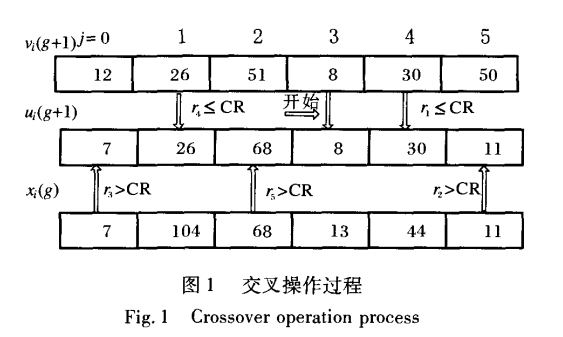
\includegraphics[width=0.8\textwidth]{fig1.png}
\end{center}
\caption{交叉操作过程}
\label{fig::fig1}
\end{figure}

\item 选择操作。DE采用贪婪算法来选择进入下一代种群的个体:
$$u_i(g+1)=
\begin{cases}
u_i(g+1) & if \quad  f(u_i(g+1)) \leq f(x_i(g))  \\
x_i(g) & otherwise
\end{cases} $$
\end{enumerate}

\subsection{差分进化算法的优缺点}
差分进化算法在求解非凸、多峰、非线性函数优化问题中表现了极强的稳健型,而且尤其擅长求解多变量的函数优化问题。并且在同样的精度要求下,由于差分进化算法具有方向性,因而收敛速度快。此外,差分进化算法操作简单,易编程实现。

然而,由于差分进化算法关键步骤变异操作是基于群体的差异向量信息来修正各个体的值,随着进化代数的增加,各个体之间的差异化信息在逐渐缩小。以至于后期收敛速度变慢,甚至有时会陷入局部最优点。

\subsection{差分进化算法的改进}
传统差分进化算法的性能很大部分的由所选择的测试向量生成策略以及相关参数值决定。如果策略及参数选择不合适,则可能产生早熟。在过去关于差分进化算法的研究中已经介绍了多种关于选择策略及参数的参考方法。

\subsubsection{改进DE的操作算子}
Ronkkonen等人提出了将参数F的初值设定为0.9,变动范围设定为[0.4,0.95]。同时CR应在[0,0.2]中取值,此时参数之间是独立的。然而在真实问题中,问题的许多特征都是无法得知的,因此选择CR值也是一件较为困难的事。Kaelo等利用竞标赛竞争选择机制来选取进行变异操作的父代基向量,同时在试验个体和种群内最好个体之间的区域,利用反射和收缩操作来实施局部搜索。Lee等提出一种基于适应性步长的局部搜索来确定合适的缩放比例因子,从而加速算法搜索的进程。Price等提出了一种试验向量生成策略DE/current-to-rand/1,并且将参数设定为NP=20D,K=0.5,F=0.8。当发生早熟时,则增大NP和F,或是减小K。当种群发生停滞现象时,则增大NP或F,或是在[0,1]中随机设定K。

\subsubsection{自适应方法}
Omran等介绍了自适应的缩放因子F以及交叉概率CR,其自适应的策略是类似的。每个个体的初始交叉概率服从正态分布N(0.5,0.15)。此方法(名为SDE)在四个基准函数上进行测试,并且表现优于其他DE。除了使F和CR可以自适应外,Teo提出一种自适应种群的微分演化(DESAP)。Brest等将个体的参数F和CR进行编码并用两种新的参数t1和t2来对参数进行调整。他们讲F的不同值组成的集合赋值给种群中的个体,并且一个变量rand从[0,1]随机生成。如果rand小于t1,则F将重新在[0.1,1.0]进行随机初始化,否则其值不变。CR的适应规则与F相同,但其初始化范围为[0,1]。

\subsubsection{多种群}
Qing将DE分成多个自种群,各个子种群独立寻优,同时利用跨种群间的竞争算子来实现种群间信息共享,并利用该算法来解决多个超导柱体电磁反转散射问题。Zaharie提出了多种群DE,并用于求解多极值的优化问题。

\subsection{差分进化算法的应用}
传统差分进化算法的性能很大部分的由所选择的测试向量生成策略以及相关参数值决定。如果策略及参数选择不合适,则可能产生早熟。在过去关于差分进化算法的研究中已经介绍了多种关于选择策略及参数的参考方法。

\subsubsection{人工神经网络}
Liu等将PSO,DE与混沌搜索相结合来训练多层前馈神经网络;Abbass利用基于BP和DE学习的神经元网络来预测乳腺癌。应用结果均显示,利用DE神经元网络是一种快速、高速并具有潜力的方法。

\subsubsection{化工领域}
Kiranmai等利用DE确定固定薄膜生物反应器的机理参数。Kapadi等利用DE解决间歇发酵最优控制和参数选择问题。Lee等提出一种基于改进DE的动态优化方法来确定连续甲基异丁烯酸盐和乙烯基醋酸盐共聚反应过程的最优控制变量轨迹,从而最小化反应启动时间和等级变化操作的过渡时间。Wang等将间歇燃料酒精发酵过程的最优加料策略转变为一个模糊决策分析问题,同时利用混合DE解决上述的最大化决策问题,求得最优加料策略。

\subsubsection{信号处理领域}
Storn利用DE设计滤波器。Shan等利用基于DE的频率域模型优化超宽带无线电系统的源脉冲和探测模型,使得自由空间的功率和接收端的相关检测输出最大。Caorsi等利用混合整数编码的DE优化设计单脉冲天线的差异模式。Yang等利用DE确定静态激励幅度分布,从而有效地降低了相中心移动天线阵的带内旁瓣电平。Li等利用DE和Newton-Raphson法,通过电阻抗X线断层摄影来重建脑部图像。

\section{总结}
本文简述了进化算法的概念、分类和流程,并重点介绍了差分进化算法。其中首先介绍了标准差分进化算法,并介绍了不同的改进方法来弥补差分进化后期收敛变慢的缺点。最后,本文介绍了差分进化算法在不同领域中的应用。

\end{document}

